\documentclass[a4paper,12pt]{article}
\usepackage[brazil]{babel}
\usepackage[utf8]{inputenc}
\usepackage{amsmath}
\usepackage{amssymb}
\usepackage{graphicx}
\usepackage{enumitem}
\usepackage{booktabs}
\usepackage{hyperref}
\usepackage{geometry}
\geometry{margin=1in}
\begin{document}

\section*{Modelo Probabilístico para um esquema de pirâmide }


Esquemas de pirâmide são frequentemente oferecidos sob o disfarce de
franquias comerciais. Um caso emblemático é o da empresa \emph{Koscot
  Interplanetary Cosmetics}, acusada pelas agências reguladoras
norte-americanas (FTC, SEC e estaduais) de operar um esquema desse
tipo, causando um prejuízo estimado em 44 milhões de dólares.  A
proposta da Koscot era que os participantes poderiam vender cosméticos
de porta em porta. No entanto, o foco da empresa estava mais na venda
de contratos de distribuição que nos cosméticos propriamente ditos. Um
contrato era vendido por US\$5.000. Os participantes também podiam
pagar US\$2.000 para se tornarem supervisores ou US\$5.400 para se
tornarem diretores. Esses níveis, em teoria, permitiriam que os
participantes ganhassem dinheiro recrutando outras pessoas para atuarem
nos níveis abaixo deles, pagando comissões sobre os pedidos de
cosméticos àqueles nos níveis superiores que os recrutaram. Esses novos
recrutas, por sua vez, recrutariam outros participantes para ganhar
comissões por conta própria. Como colocou uma matéria jornalística:
\begin{quotation}
  Pense nisso: uma pessoa poderia vender 10 distribuições, e cada uma
  dessas 10 poderia vender mais 10, e assim por diante. Os
  distribuidores poderiam ganhar milhares de dólares. O sujeito no topo
  poderia ganhar milhões. \dots Turner tinha um talento para fazer as
  pessoas acreditarem nele. Seus encontros de vendas se tornaram
  lendários. \dots Nas reuniões, os protegidos de Turner corriam para o
  palco com seus ternos chamativos e sapatos elegantes, com notas de
  \$100 ou até \$1.000 presas às lapelas. Eles dirigiam Cadillacs novos
  e usavam sapatos de couro de jacaré. ``E você também pode'', diziam à
  plateia. ``Tudo o que você precisa fazer é acreditar.'' \emph{Orlando
    Sentinel}, 17/08/1987.
\end{quotation}

Os promotores oferecem remuneração em vendas, mas a maior parte do
lucro vem do recrutamento de novos vendedores, e não da venda de
produtos.

O problema mais básico aqui é a \textbf{explosão exponencial}. Se fosse
verdade que cada participante conseguisse recrutar, por exemplo, duas
pessoas por mês, em cerca de 27 meses toda a população (atual) do
Brasil estaria envolvida, o que é claramente impossível. Esse argumento
utiliza o crescimento geométrico para mostrar a insustentabilidade do
esquema. No entanto, tribunais às vezes rejeitam essa visão como
irrealista \cite{gerro_mar}. Para evitar essas críticas, operadores
definem cotas geográficas para limitar o recrutamento.


\paragraph{Exemplo legal: o caso do \textit{Golden Book of Values} em
  Connecticut \cite{naruk}}

Outro ilustra como um empreendimento comercial legítimo pode se
misturar a um esquema de pirâmide.
\begin{itemize}[noitemsep]
\item Os franqueados pagavam uma taxa de US\$2.500 para obter uma
  franquia do \textit{Golden Book of Values}.
\item Havia duas formas principais de ganho:
  \begin{enumerate}[label=(\alph*),noitemsep]
  \item Desenvolver um ``Book of Values'' local para venda ao público:
    \begin{itemize}
    \item Vendendo anúncios para comerciantes a US\$195 cada, recebendo
      50\% de comissão.
    \item O livro continha entre 50 e 100 ofertas de descontos e era
      vendido por US\$15, dos quais o franqueado recebia US\$12.
    \end{itemize}
  \item Recrutar novos franqueados, recebendo US\$900 por cada novo
    recrutamento.
  \end{enumerate}
\end{itemize}

Como a produção e venda do livro exigiam tempo, o recrutamento se
tornava claramente a fonte mais lucrativa. A brochura de recrutamento
prometia ganhos elevados, ilustrando o seguinte cenário: se o
franqueado inscrevesse duas pessoas por mês, após um ano ganharia
US\$21.600 só com recrutamento.

\textbf{A acusação} questionou a validade dessa previsão:
\begin{itemize}[noitemsep]
\item Supondo que cada franqueado realmente inscreva dois novos por
  mês, o número de franqueados cresceria em progressão geométrica
  triplicando a cada mês.
\item O professor Margolin (Yale) testemunhou que em 18 meses toda a
  população dos EUA estaria envolvida, o que é impossível.
\item Logo, a estimativa da brochura era enganosa, pois a maioria não
  poderia alcançar esses ganhos.
\end{itemize}

O esquema possuía uma nuance estatística adicional:
\begin{itemize}[noitemsep]
\item Havia uma cota de 270 franquias para todo o estado de
  Connecticut.
\item O tribunal observou que, com essa cota e o recrutamento de dois
  novos por mês, apenas 27 franqueados conseguiriam lucrar, enquanto os
  outros 243 perderiam dinheiro.
\end{itemize}

\subsection*{Modelo probabilístico}

Como o recrutamento real não segue um padrão tão
regular — ou seja, nem todos recrutam dois novos membros por mês — a
próxima etapa é desenvolver um modelo probabilístico para entender
melhor o comportamento do esquema. Esse modelo permite:
\begin{itemize}[noitemsep]
\item Calcular a distribuição de probabilidade do número de pessoas
  recrutadas por cada participante.
\item Analisar como a chance de recuperar o investimento inicial
  depende do momento em que o participante entra no esquema.
\item Determinar a fração de participantes que não conseguirão recrutar
  ninguém.
\end{itemize}
Para ações legais, é mais útil uma {afirmação absoluta} de que a
probabilidade de recuperar o investimento é pequena, do que uma simples
estimativa aproximada. O modelo probabilístico para esses esquemas de
pirâmide apresenta resultados quantitativos para o comportamento dos
participantes:
\begin{itemize}[noitemsep]
\item A maioria dos participantes tem \textbf{menos de 10\% de chance}
  de recuperar o investimento inicial, assumindo um pequeno lucro ao
  recrutar três pessoas.
\item Em média, \textbf{metade dos participantes não recruta ninguém} e
  perde todo o dinheiro investido.
\item Cerca de \textbf{1 em 8 participantes recruta três ou mais
    pessoas}.
\item Menos de \textbf{1\% dos participantes pode esperar recrutar seis
    ou mais pessoas}.
\end{itemize}

Vamos assumir um esquema de recrutamento com cota:
\begin{itemize}[noitemsep]
\item $c$ é o custo para entrar em um esquema de pirâmide;
\item $d$ é o bônus por recrutamento;
\item $N$ é o limite de participantes.
\end{itemize}

Denotamos por $R$ o número esperado de pessoas recrutadas por um
participante. Um pessoa deve participar do esquema de $$R\cdot d > c$$
ou seja, se os ganhos esperados $Rd$ superarem o custo de entrada.

\subsection*{Número esperado de recrutas para o participante $k$}

No momento em que há $k$ participantes tentando recrutar não há motivo,
por construção, para que um participante tenha mais ou menos chance de
recrutar do que os outros. Vamos assumir que o próximo participante é
escolhido por qualquer um dos atuais com probabilidade $\tfrac 1k$,
para todo $k=1,2,\dots,N-1$.

Nesse momento, o número de recrutamentos pelo $k$-ésimo recrutado (que
ainda não recrutou ninguém) é a variável aleatória
\[
  S_k = \sum_{i=k}^{N-1} X_i, \text{ onde }
  X_i = 
  \begin{cases}
    1, & \text{ com probabilidade } p_i= \tfrac 1i,\\
    0, & \text{ com probabilidade } 1- \tfrac 1i,
  \end{cases}
\]
e o valor esperado de recrutamentos é dado por
\begin{equation}
  \mathbb E[S_k] = \sum_{i=k}^{N-1} \frac{1}{i}.
\end{equation}
O $n$-ésimo número harmônico tem a seguinte
aproximação\footnote{$H_n = \ln n + \gamma + \frac{1}{2n} -
  \frac{1}{12n^2} + \frac{1}{120n^4} - \cdots $.}
\[
  H_n= \sum_{i=1}^n \frac 1i = \ln n+ \gamma  + \omega(n) 
\]
onde $\gamma\approx 0,577$ é a
\href{http://en.wikipedia.org/wiki/Euler\%E2\%80\%93Mascheroni_constant}{constante
  de Euler--Mascheroni} e $\omega(n)$ tende a $0$ quando $n\to \infty$,
ou seja, $H_n - \ln(n) \to \gamma$.

Disso,
\[
  \sum_{i=k}^{N-1} \frac{1}{i} =
  \sum_{i=1}^{N-1} \frac{1}{i} -
  \sum_{i=1}^{k-1} \frac{1}{i}
  \approx
  \ln(N-1) - \ln(k-1) 
\]
logo
\begin{equation}\label{eq:harmonico}
  \mathbb E[S_k]  \approx\ln\left( \tfrac{N-1}{k-1}\right).
\end{equation}

Isso implica que,
\begin{center}
  \begin{minipage}[h]{.9\linewidth}
    \emph{para $k \geq \frac{N}{e} \approx 0{,}37N$, o participante
    pode esperar recrutar não mais que \emph{uma pessoa}. Portanto,
    apenas os primeiros 37\% dos participantes têm chance razoável de
    recrutar ao menos um novo membro.}\end{minipage}
\end{center}



\subsection*{Probabilidade de recrutar pelo menos
  $\left\lceil \frac{c}{d} \right\rceil + 1$ pessoas}

Para obter lucro, o participante deve recrutar pelo menos
\[
b = \left\lceil \frac{c}{d} \right\rceil + 1
\]
pessoas.  Por exemplo, se $c=2500$ e $d=900$ então $b=3$ e devemos
estimar \(\mathbb P(S_k \geq 3)\). Uma possibilidade é usarmos uma
aproximação de Poisson, outra é calcular numericamente, já que não há
uma fórmula fechada para determinar ao menos um limitante superior
para
\[
  \mathbb P(S_k \geq b) = p(b) + p(b+1)+\cdots+p(N-k)
\]
onde $p(x) = \mathbb P(S_k=x)$ é a função de massa de probabilidade (fmp) de
$S_k$. Podemos calcular essa probabilidade usando convolução [código em
python
\href{https://colab.research.google.com/drive/1ny7iBL4APXU2uY0w2B4Pfw0gVBnoZD3w#scrollTo=GRPo2NvLSWOe}{clique
  aqui}].  Queremos calcular a distribuição de probabilidade exata de
\( S_k = \sum_{i=k}^{N-1} X_i \), onde as variáveis \( X_i \) são
independentes e
\( X_i \sim \mathrm{Bernoulli}\left(\tfrac{1}{i}\right) \). Para isso,
utilizamos convoluções sucessivas de distribuições de Bernoulli.

\fbox{
  \begin{minipage}[h]{1.0\linewidth}
    
    \textbf{Exemplo.} Seja
    \[
      S_k = X_k + X_{k+1} + X_{k+2},
    \]
    com \(X_k \sim \mathrm{Bernoulli}(p_k)\),
    \(X_{k+1} \sim \mathrm{Bernoulli}(p_{k+1})\),
    \(X_{k+2} \sim \mathrm{Bernoulli}(p_{k+2})\), e
    \(p_i = \frac{1}{i}\). Todos os \(X_i\) são independentes.
    
    \begin{enumerate}[noitemsep]
    \item A distribuição de \(X_k\) é:
      \[
        f_{X_k}(s) =
        \begin{cases}
          1 - p_k, & \text{se } s = 0, \\
          p_k,     & \text{se } s = 1.
        \end{cases}
      \]
      
    \item A soma \(S^{(1)} = X_k + X_{k+1}\) tem distribuição dada pela
      convolução:
      \[
        f_{S^{(1)}}(s) = (f_{X_k} * f_{X_{k+1}})(s)
        = \sum_{j=0}^s f_{X_k}(j) \cdot f_{X_{k+1}}(s - j),
      \]
      que resulta em
      \begin{align*}
        f_{S^{(1)}}(0) &= (1 - p_k)(1 - p_{k+1}), \\
        f_{S^{(1)}}(1) &= (1 - p_k)p_{k+1} + p_k(1 - p_{k+1}), \\
        f_{S^{(1)}}(2) &= p_k p_{k+1}.
      \end{align*}
      
    \item Agora somamos \(X_{k+2}\): \(S_k = S^{(1)} + X_{k+2}\). A
      nova distribuição é:
      \[
        f_{S_k}(s) = (f_{S^{(1)}} * f_{X_{k+2}})(s)
      = \sum_{j=0}^s f_{S^{(1)}}(j) \cdot f_{X_{k+2}}(s - j)\]
      com:
      \begin{align*}
        f_{S_k}(0) &= f_{S^{(1)}}(0) \cdot (1 - p_{k+2}), \\
        f_{S_k}(1) &= f_{S^{(1)}}(0) \cdot p_{k+2} + f_{S^{(1)}}(1) \cdot (1 - p_{k+2}), \\
        f_{S_k}(2) &= f_{S^{(1)}}(1) \cdot p_{k+2} + f_{S^{(1)}}(2) \cdot (1 - p_{k+2}), \\
        f_{S_k}(3) &= f_{S^{(1)}}(2) \cdot p_{k+2}.
      \end{align*}
      
    \item Assim, a função de massa de probabilidade final de \(S_k\) é:
      \[
        f_{S_k}(s) = \mathbb{P}(S_k = s), \quad \text{para } s = 0, 1,
        2, 3.
      \]
      
    \item Finalmente, a probabilidade que desejamos é:
      \[
        \mathbb{P}(S_k \geq b) = \sum_{s =  b }^{3} f_{S_k}(s).
      \]
    \end{enumerate}
    
  \end{minipage}
}

  

Nosso objetivo é calcular a distribuição exata de
\[
S_k = X_k + X_{k+1} + \cdots + X_{N-1},
\]
onde \(X_i \sim \mathrm{Bernoulli}(p_i)\), com \(p_i = \frac{1}{i}\), e as variáveis \(X_i\) são independentes.

Vamos construir a função de massa de probabilidade (fmp) de \(S_k\) de forma iterativa, usando convoluções.

\begin{enumerate}
  \item Começamos com a distribuição de \(X_k\):
  \[
  f_{X_k}(s) =
  \begin{cases}
    1 - \tfrac{1}{k}, & \text{se } s = 0, \\
    \tfrac{1}{k},     & \text{se } s = 1.
  \end{cases}
  \]
  Denotamos essa fmp como \(f^{(k)}_1(s)\), a distribuição da soma parcial \(S_k^{(1)} = X_k\).

  \item Em seguida, somamos \(X_{k+1}\): a distribuição de \(S_k^{(2)} = X_k + X_{k+1}\) é dada por:
  \[
  f^{(k)}_2(s) = (f_{X_k} * f_{X_{k+1}})(s) = \sum_{j=0}^{s} f_{X_k}(j) \cdot f_{X_{k+1}}(s - j),
  \]
  onde \(f_{X_{k+1}}(0) = 1 - \tfrac{1}{k+1}\), \(f_{X_{k+1}}(1) = \tfrac{1}{k+1}\).

  \item Continuamos esse processo iterativamente. Para cada \(i = k+2, \dots, N-1\), definimos:
  \[
  S_k^{(i - k + 1)} = X_k + X_{k+1} + \cdots + X_i,
  \]
  e atualizamos a distribuição:
  \[
  f^{(k)}_{i - k + 1}(s) = (f^{(k)}_{i - k} * f_{X_i})(s),
  \]
  onde \(f_{X_i}(0) = 1 - \tfrac{1}{i}\), \(f_{X_i}(1) = \tfrac{1}{i}\).

  \item Após a última convolução com \(X_{N-1}\), obtemos a distribuição de
  \[
  S_k = X_k + X_{k+1} + \cdots + X_{N-1},
  \]
  com fmp final denotada por \(f^{(k)}(s)\).

  \item Finalmente, a probabilidade que queremos calcular é:
  \[
  \mathbb{P}(S_k \geq b) = \sum_{s =  b }^{N - k} f^{(k)}(s),
  \]
  onde \(f^{(k)}(s)\) é a probabilidade de \(S_k = s\), computada via
  as convoluções acima.
\end{enumerate}



A Tabela \ref{tab:probabilidades} mostra algumas essas probabilidades
para $N=270$, confirmando que a chance de recuperar o investimento
diminui rapidamente conforme o esquema avança. A tabela completa está
\href{https://docs.google.com/spreadsheets/d/1xrFkBaQD_7dD_BXeq6PeXPoeMQ9u4H8-G-ZwPQcySSI/edit?usp=sharing}{aqui}.

\begin{table}[htbp]
    \centering
    \caption{Número esperado de recrutamentos e limites superiores para
      a probabilidade de recrutar pelo menos 2 ou 3 membros
      ($N=270$).}\label{tab:probabilidades}
    \begin{tabular}{ccc}
      \toprule
      Posição $k$ & Número esperado de recrutados & Probabilidade de $\geq r$ recrutados \\
                  & & $r=2$ \quad $r=3$ \\
      \midrule
      5   & 4{,}21 & 0{,}92 \quad 0{,}79 \\
      10  & 3{,}40 & 0{,}85 \quad 0{,}66 \\
      20  & 2{,}65 & 0{,}74 \quad 0{,}49 \\
      30  & 2{,}23 & 0{,}65 \quad 0{,}38 \\
      50  & 1{,}69 & 0{,}51 \quad 0{,}24 \\
      60  & 1{,}51 & 0{,}45 \quad 0{,}19 \\
      70  & 1{,}36 & 0{,}39 \quad 0{,}16 \\
      80  & 1{,}22 & 0{,}35 \quad 0{,}12 \\
      90  & 1{,}10 & 0{,}30 \quad 0{,}10 \\
      100 & 1{,}00 & 0{,}26 \quad 0{,}08 \\
      110 & 0{,}90 & 0{,}23 \quad 0{,}06 \\
      120 & 0{,}81 & 0{,}20 \quad 0{,}05 \\
      130 & 0{,}73 & 0{,}17 \quad 0{,}04 \\
      140 & 0{,}66 & 0{,}14 \quad 0{,}03 \\
      150 & 0{,}59 & 0{,}12 \quad 0{,}02 \\
      240 & 0{,}12 & 0{,}01 \quad 3{,}0$\times10^{-4}$ \\
      260 & 0{,}03 & 6{,}3$\times10^{-4}$ \quad 6{,}3$\times10^{-6}$\\
      \bottomrule
\end{tabular}
\end{table}

  
\bigskip

\subsection*{Retorno esperado para o grupo dos participantes}

Para $K$ participantes inscritos, o lucro líquido do promotor (primeiro
participante) é
\[
  L = \underbrace{(K-1)c}_{\text{recebe}} -
  \underbrace{(K-2)d}_{\text{paga}} = c + (K-2)(c - d).
\]
A fração do investimento total devolvida aos participantes é
aproximadamente
\[
\frac{(K-2)}{(K-1)} \times \frac{d}{c} \approx \frac{d}{c}.
\]
Portanto, a parte do dinheiro investido que retorna aos participantes é
um pouco menor do que $d/c$, ou seja, a razão entre o valor recebido
por cada recrutamento e o investimento inicial. No caso ilustrado
($c=2500$ e $d=900$), esse valor é de apenas $9/25 = 0{,}36$. Assim,
como um grupo, os participantes perdem 64\% do investimento.


\subsection*{Metade dos participantes não recrutam ninguém}

A probabilidade do $k$-ésimo participante não recrutar ninguém é
\[
  P_k(0) = \prod_{i=k}^{N-1} \left(1 - \frac{1}{i}\right) =
  \frac{k-1}{N-1}.
\]
Assim, o número esperado de participantes que não recrutam ninguém é
\[
  \mathbb E[\text{número de não recrutadores}] = \sum_{k=1}^{N} P_k(0)
  = \frac{N-1}{2} \approx \frac{N}{2}.
\]
Portanto, em média, metade dos investidores perde todo o dinheiro
investido. Importante notar que isso vale independentemente de $d$,
\emph{mesmo que todo dinheiro arrecadado fosse distribuído, metade não
  receberia nada.}

\subsection*{Distribuição assintotica do número de recrutamentos}

Pode-se questionar a relevância desse resultado em um processo judicial
se um número significativo de participantes obtivesse altos
retornos. Entretanto, podemos mostrar que a fração dos participantes
que recrutam exatamente $r$ pessoas se aproxima de $2^{-(r+1)}$ à
medida que $N$ cresce. Consequentemente, a fração dos participantes que
recrutam pelo menos $r$ membros é aproximadamente $2^{-r}$. Isso
implica que:
\begin{itemize}[noitemsep]
\item Apenas 1/8 dos participantes pode esperar recrutar pelo menos 3
  membros.
\item Apenas 1 em 16 milhões pode esperar recrutar 24 ou mais membros.
\end{itemize}

Este modelo confirma o julgamento do caso Golden Book of Values,
reforçando a impossibilidade de ganhos conforme a propaganda. Como
consequência, o juiz proibiu permanentemente os réus de continuar a
venda das franquias ou iniciar novos esquemas similares sem aprovação
judicial.

\subsubsection*{Ideia: caminhos da aproximação}
No nosso caso, temos $p_i = 1/i$, e desejamos aproximar
\begin{equation}
  {S}_{k}  = \sum_{i=k}^{N-1} X_i
\end{equation}
por uma variável de Poisson $P_k$ com parâmetro $\gamma_k$
\begin{equation}
  \gamma_k = \ln \left( \frac{N-1}{k-1} \right).
\end{equation}
Vale que
\[
  \mathbb P(S_k\geq r) \leq \sum_{i=r}^\infty \mathbb P (P_k =i)
  =1-\sum_{i=1}^{ r-1}\frac{k-1}{N-1}\cdot\frac{\gamma_k^i}{i!}.
\]
Como as variáveis $P_k$ que aproximam $S_k$ são muito próximas, podemos
derivar uma aproximação precisa para a fração esperada de participantes
que recrutarão pelo menos $r$ pessoas: \emph{sejam
  $X_2, X_3, \dots, X_N$ uma sequência de variáveis Poisson com
  parâmetros $\gamma_k$. Então,}
\begin{equation}\label{eq:(10)}
 % \frac{1}{N-1} \sum_{r=1}^{N-1} \mathbb P(S_k = r) =
  \frac{1}{N-1} \sum_{k=2}^{N-1} \mathbb P(X_k = r) \to \frac{1}{2^{r+1}}, \quad \text{para } r = 0, 1, 2, \dots
\end{equation}
\emph{quando $N \to \infty$.} Portanto, para grandes valores de $N$, a
fração esperada de participantes que recrutam pelo menos $r$ pessoas é
dada por $1/2^r$, para $r = 0, 1, 2, \dots$.

Para avaliar a rapidez com que esse limite é atingido, calculamos os
valores exatos da equação \eqref{eq:(10)} para $N = 270$ e $N = 1000$,
com $r = 1, 2, 3$. Os valores obtidos foram:
\begin{align*}
   \mathbb P(X_k \geq 1) &= 0,24991 \text{ para } N = 270, \quad 0,24999 \text{ para } N = 1000, \\
  \mathbb  P(X_k \geq 2) &= 0,12475 \text{ para } N = 270, \quad 0,12497 \text{ para } N = 1000, \\
  \mathbb  P(X_k \geq 3) &= 0,06202 \text{ para } N = 270, \quad 0,06244 \text{ para } N = 1000.
\end{align*}


\subsubsection*{Adendo: Limites para o número harmônico via aproximação
  por integral}


A função \( f(x) = \frac{1}{x} \) é contínua, positiva e decrescente
para \( x \geq 1 \). Podemos então comparar a soma que defini $H_n$ com
integrais definidas:

\medskip

\emph{Limite inferior}: Como a soma \( \sum_{k=1}^n \frac{1}{k} \) pode
ser interpretada como a soma das áreas de retângulos de base 1 e altura
\( \frac{1}{k} \), e como esses retângulos estão acima da curva
\( y = \frac{1}{x} \) no intervalo correspondente, temos:

\[
\int_1^{n+1} \frac{1}{x} \, dx = \ln(n+1) < H_n
\]

\medskip

\emph{Limite superior}: 
Separando o primeiro termo da soma \( \frac{1}{1} = 1 \), temos:
\[
H_n = 1 + \sum_{k=2}^n \frac{1}{k}
\]
como os retângulos de altura \( \frac{1}{k} \) agora estão abaixo
da curva \( y = \frac{1}{x} \) no intervalo \( [k-1, k] \), obtemos:
\[
H_n < 1 + \int_1^n \frac{1}{x} \, dx = 1 + \ln n
\]

%\begin{figure}[h!]
    {\centering
    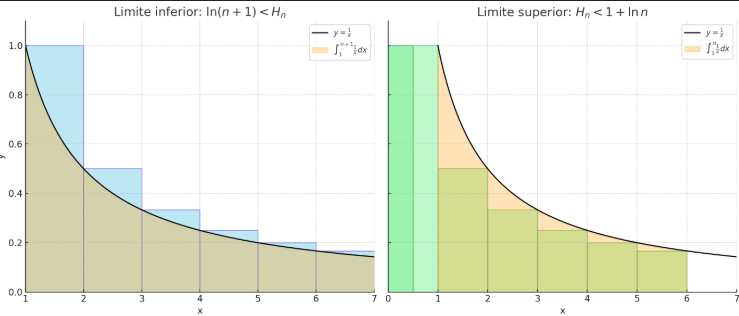
\includegraphics[width=0.85\textwidth]{harmonico.png}}
%\end{figure}

Combinando os dois resultados:
\[
\boxed{
\ln(n+1) < H_n < 1 + \ln n
}
\]





\bibliographystyle{plain}
%\bibliography{referencias} 

\begin{thebibliography}{1}

\bibitem{naruk} H.~Naruk.  \newblock Memorandum of decision: State of
  connecticut vs. bull investment group.  \newblock Technical Report 32
  Conn. Sup. 279, State of Connecticut, 1975. \newblock Resumo
  traduzido \url{https://docs.google.com/document/d/1Ya3RfXYVCbRusIMefzGNV4IaR7koQOYRkJfTELPz-Sc/edit?usp=sharing}

\bibitem{gerro_mar} Ger-ro-mar, inc.~v.~ftc, 518 f.2d 33 (2d
  cir. 1975).  \newblock
  \url{https://www.ftc.gov/legal-library/browse/cases-proceedings/7023493-ger-ro-mar-matter}.

\bibitem{conv} Wikipedia.  \newblock Convolução.
  \newblock \url{https://pt.wikipedia.org/wiki/Convolu%C3%A7%C3%A3o}.

\bibitem{poisson} Wikipedia.  \newblock Distribuição de Poisson.
  \newblock \url{https://en.wikipedia.org/wiki/Poisson_distribution}.
  \newblock Em inglês, se precisar use o google tradutor.

    
\end{thebibliography}


\end{document}
